%!TEX root = main.tex

\section{Analysis of Web Search}
\label{sec:web_search}

\begin{figure}[th]
\centering
	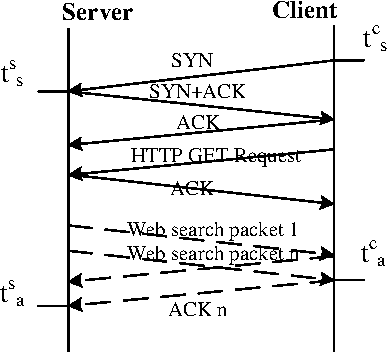
\includegraphics[width=0.5\linewidth]{web_finish_time_example}
\caption{Time-line in web search flow.}
\label{fig:web_finish_time_example}
\end{figure}

Web search starts when mobile terminal initiates connection to transmit query text, and ends when server receives ACKs for all returned search results. Figure~\ref{fig:web_finish_time_example} shows the typical time-line in web search flows. The finish time at client side is the duration from transmitting SYN packet $t^c_s$ to receiving all web search data $t^c_a$. We use the duration $T_s=t^s_a - t^s_s$ measured at server side to approximate the latency that user perceives. Again, we excluded the time consumed by servers processing the query $T_r=t^s_r - t^s_q$ and obtained the finish time as $T_s-T_r$.

For each data packet which is not retransmitted, the measured RTT is the duration from that server transmits the packet, to that server receives the acknowledgment for it. In web search progress, we record as many RTT's as possible. When each new RTT is measured, the RTO value is updated by $RTO = SRTT + max(200ms, 4 RTTVAR)$, where $SRTT$ and $RTTVAR$ mean smoothed RTT and RTT variation respectively. For a retransmitted packet, if the duration between its retransmission time and the time that last packet is transmitted is larger than the calculated RTO, we could infer that it is a timeout retransmission. For each retransmitted packet, if server would not receive D-SACK, such a retransmission recovers a real packet loss, otherwise, the packet is not dropped and the retransmission is spurious. Note that a data segment could be retransmitted twice or more if the previously retransmitted packet is regarded as lost.

In the above, we have seen that finish time in voice recognition is strongly related to the RTT value. Here we investigate the impact of RTT on finish time of web search flows. The distribution of RTT in web search is similar to that in voice recognition, which is not shown due to space limit. We use Kendall correlation to determine their relationship. The coefficient between RTT and finish time is 0.15, showing weak relationship between them. The reason is as follows. Web search result usually contains more than 10 data packets (shown in Figure~\ref{fig:web_flow_size}), which could be transmitted in 1 RTT. Moreover, how many data packets could be transmitted in one RTT is determined by congestion window size, which varies when receiving acknowledgment and packet loss event. Flows have different congestion window sizes due to different amount of congestion events in the paths they traverse. Thus RTT has limited impact on finish time in web search. 

\begin{figure}[th]
\centering
	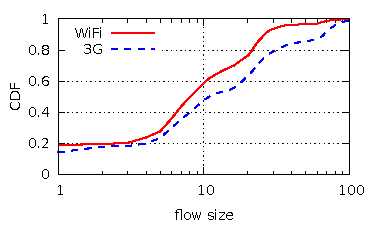
\includegraphics[width=0.8\linewidth]{web_flow_size}
\caption{The distribution of flow sizes in web search.}
\label{fig:web_flow_size}
\end{figure}

Figure~\ref{fig:web_flow_size} plots the distribution of flow size (measured by the number of web search result packets) in web search. The flow size varies from 1 packet to 100 packets with a median around 10 packets. Such a small flow size implies that any TCP performance degradation (like a high packet loss) could exert a large impact on the user perceived latency (i.e. finish time) \cite{flach2013reducing}. We also observe a smaller flow size of WiFi search than that of 3G search, which might be due to the difference in search behavior \cite{Song:2013:EEU:2488388.2488493}. We use Kendall correlation to determine whether flow size is relevant to finish time. The coefficient is 0.018, which demonstrates their irrelevance.

As a TCP sender in web search, the server can measure abundant TCP performance factors and behavior, enabling us to perform a detailed analysis of the TCP performance and its impact on the finish time. In what follows, we first characterize the finish time distribution in 3 TCP stages and then examine the impact of TCP performance factors.

\subsection{TCP Stage Analysis}

\begin{figure}[th]
\centering
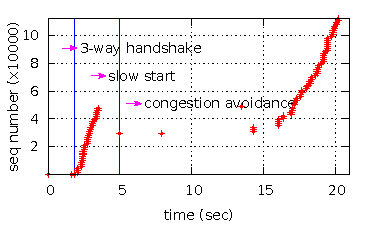
\includegraphics[width=0.8\linewidth]{web_three_stages}
\caption{The three stages in web search flows.}
\label{fig:web_three_stages}
\end{figure}

A TCP comprises 3 stages: \emph{3-way handshake}, \emph{slow start}, \emph{congestion avoidance}, which is exemplified in Figure~\ref{fig:web_three_stages} using a web search flow from our dataset, where $y$-axis shows the TCP sequence number. The TCP 3-way handshake (3WHS) stage ideally (i.e. without packet loss, delay and reordering) completes within 1 RTT. The server then enters the slow start stage, during which server does not encounter any packet loss or reordering event, and thus enlarges the congestion window by 1 segment size for each received ACK. The server enters congestion avoidance stage once it estimates a packet loss\footnote{The packet can actually be delayed or lost.}. In this stage, the server reduces the congestion window when detecting packet loss through fast retransmit\cite{jacobson1988congestion} and compels the congestion window to grow from 1 segment size when detecting packet loss through RTO. Note that the congestion avoidance stage here starts when server detects congestion event and ends till the flow finishes, which is different the TCP congestion avoidance state in TCP/IP stack.

%Figure~\ref{fig:web_three_stages} gives an exemplified flow with 3 TCP stages that we define. The $y$-axis shows the TCP sequence number. In the figure, server takes 1.8s to establish connection, 3.1s to transmit 35 data packets in slow start stage, and 15.3s to transmit the left 48 data packets in congestion avoidance stage. In the following, we use the criteria of partitioning to break the analysis down into the three stages that flows experience.

\subsubsection{3-way Handshake}

\begin{figure}[th]
\centering
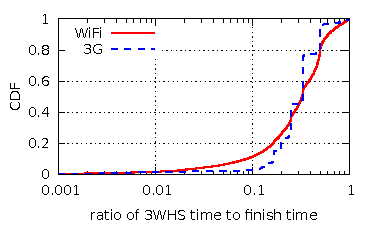
\includegraphics[width=0.8\linewidth]{web_handshake_time_ratio}
\caption{The ratio of time in 3-way handshake to finish time in each flow.}
\label{fig:web_handshake_ratio}
\end{figure}

We first examine how much of the time spent in the 3WSH stage in Figure~\ref{fig:web_handshake_ratio}, where we plot the ratio of the time in 3WSH to the finish time. 3G and WiFi show similar ratio of time spent in this stage. We observe that the time for connection establishment can take up to half of the finish time for 30\% flows. More surprisingly, about 8\% of the WiFi flows and 3\% of 3G flows spend 70\% of their time during this stage. The small flow size is one of the reason for this observation. The maximum flow size is around 100 packets as shown in Figure \ref{fig:web_flow_size}, implying the data can be transmitted within only a few RTTs if no congestion event happens. such a short period of transmission time leads to a relatively large portion of time for connection establishment.


%From the figure, flows in cellular network have similar ratio of time in 3-way handshake to that in WiFi network (with median value 0.3). If the 3WSH could be removed from finish time, the user-perceived web search latency would be reduced by 30\% in more than half of the flows. Moreover, there are 8\% of flows in WiFi network consuming 70\% of their time in 3WSH.

%The unexpectedly high ratio of 3WSH could be introduced by two reasons. First, most of web search flows contains packets ranging from 1 to 100, these data could transmitted in 1 to 4 RTT's if there is no congestion event. Thus 3WHS, without transmitting any data, occupies a large fraction of time in short flows. Second, there are a non-negligible fraction of flows experiencing SYN retransmission during 3WHS stage. 

Another important reason that explains the unexpectedly the long time in 3WSH stage (i.e. $>70\%$ of finish time) is the timeout retransmissions in this stage. As the data cannot be transmitted before a TCP connection is established, a loss of SYN will lead to a timeout retransmission, which takes 1 second (\ie the initial RTO) to retransmit the SYN.  We find that 4.4\% of WiFi search flows and 0.5\% of 3G flows experience at least one SYN timeout retransmission. We envision a possible way to mitigate the costly 3WSH in such short flows where clients maintain long-term TCP connections to the web search servers.

\subsubsection{Slow Start Stage}

\begin{figure}[th]
\centering
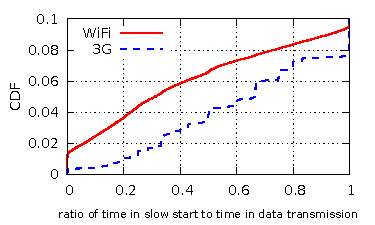
\includegraphics[width=0.8\linewidth]{web_slowstart_time_ratio}
\caption{The ratio of time in slow start to the time in data transmission.}
\label{fig:web_ss_time_ratio}
\end{figure}

The slow start stage and the congestion avoidance stage constitute the data transmission period. During the slow start stage, the data transmission throughput monotonically increases as the congestion window is doubled after each RTT. Intuitively, a longer time in slow start stage, the shorter time to complete the data transmission. Figure~\ref{fig:web_ss_time_ratio} shows the ratio of time in slow start stage to the time spent in data transmission (\ie the sum of time in slow start and congestion avoidance stages). Note that the $y$-axis is capped at 0.1. Regardless of the access type, more than 90\% of the flows can be finished in the slow start stage. In other words, about 10\% of the flows have to experience the congestion avoidance stage, which could lead to an increased finish time as we will see in the following analysis.

Another interesting observation is that 1.5\% of the WiFi flows is unable to transmit any data in the slow start stage as the first packet is dropped. We indeed find of the flows that experience the congestion avoidance stage, the packet loss happens within the first congestion window (i.e. within the first 10 packets) for 80\% of WiFi flows, while this percentage is only 20\% for 3G flows, implying a reconsideration of the initial congestion window configuration.

\subsubsection{Congestion Avoidance Stage}

\begin{figure}[th]
\centering
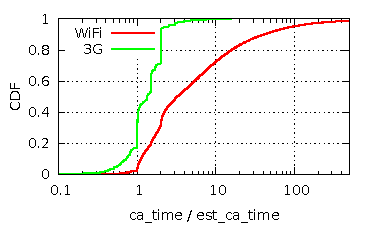
\includegraphics[width=0.8\linewidth]{web_ca_prac_over_est}
\caption{CDF of the extra time introduced by the congestion avoidance stage.}
\label{fig:web_ca_round}
\end{figure}

We then examine how much extra time the congestion avoidance stage introduces for individual flows. To this end, we first compute an estimated ideal transmission time ($T_e$) without this stage for each flow. The estimated ideal time is $T_e = \frac{\#(ca\_pkts)}{cwnd} \times RTT$, where $\#(ca\_pkts)$ is the number of packets transmitted in this stage, $cwnd$ is the congestion window size at the server at the time when entering this stage. However, we cannot obtain $cwnd_e$ from the traces and thus alternatively use the number of in-flight packets at the time when entering the stage to approximate $cwnd_e$ \cite{rfc56812009tcp}. Then we compute the ratio of the time spent in this stage obtained from the trace (denoted as $T_r$) to the estimated idea transmission time. We use this ratio to measure the extra time introduced by the congestion avoidance stage and show the results in Figure \ref{fig:web_ca_round} for those flows experiencing this stage.

We observe a surprisingly high ratio for WiFi flows. The median ratio is as high as 3.2 and 20\% of the WiFi flows has a ratio more than 11, meaning a 10 times extra time is introduced by this stage. The high ratio can be attributed to two factors. First, the real congestion window of these flows is much smaller than $cwnd_e$ due to packet losses. Second, some lost packets require the timeout retransmission to recover, in which cases server must wait for a RTO without data transmission. It is interesting to see that 3G flows have a ratio no more than 2 for 95\% of the flows, meaning that 3G flows have a low packet loss rate and experience fewer timeout retransmissions. In what follows, we will examine in detail the impact of packet loss and timeout retransmission on finish time. 

\subsection{Impact of packet loss}
\label{sec:web_pkt_loss}

% \begin{figure}[th]
% \centering
% 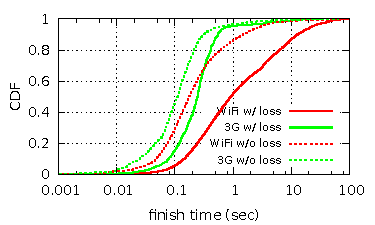
\includegraphics[width=0.8\linewidth]{web_loss_fintime_cdf}
% \caption{The distribution of finish time with and without packet loss in web search.}
% \label{fig:web_loss_fintime_cdf}
% \end{figure}

As we have analyzed above, packet loss would degrade TCP performance by both reducing congestion window and possibly triggering timeout retransmission. The the web search dataset, about 9\% of flows in both WiFi and 3G network experience packet loss. However, the packet loss rates in WiFi and 3G network are 3\% and 0.9\% respectively.

% Figure~\ref{fig:web_loss_fintime_cdf} shows the distribution of finish time with and without packet loss in web search. In the figure, there are distinct performance gap between flows with and without packet loss. The mean finish time in flows without packet loss is about 2.5 - 5 times smaller than that of flows with packet loss.

\begin{figure}[th]
\centering
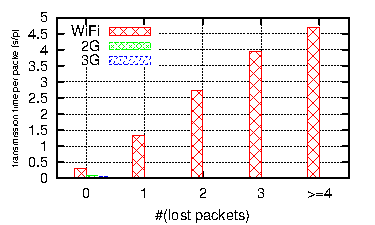
\includegraphics[width=0.8\linewidth]{web_loss_finish_time}
\caption{Finish time under different number of lost packets.}
\label{fig:web_loss_finish_time}
\end{figure}

To quantitatively determine the impact of packet loss, we investigate how much packet loss events could increase finish time. Figure~\ref{fig:web_loss_finish_time} shows the finish time of web search flows under different number of lost packets. In the figure, flows are grouped by counting how many lost packets in each flow, and the average finish time, as well as 5 and 95 percentile of finish time in each group are calculated. When there is no packet loss, the average finish time of flows in WiFi network is about 1 second, while that of flows in 3G network is only 0.3 second, which is induced by smaller RTT in 3G network. When the number of lost packets is 1 or 2, the finish time in WiFi network increases to about 2.7 second, while that of flows in 3G network hardly increases, compared with those without packet loss. When the number of lost packets increases to 3 or more, the finish time in WiFi increases to 8.1 second, while that in 3G network increases to 0.51 second. Thus, compared with flows in 3G network, flows in WiFi experience much longer finish time under the same level of packet loss, and will suffer more severe performance degradation if the number of lost packets increases. 

\subsection{Impact of timeout retransmission}

\begin{figure}[th]
\centering
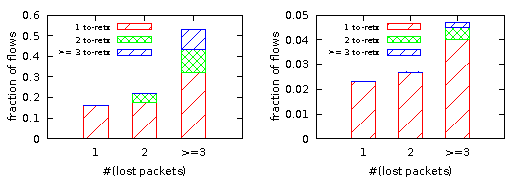
\includegraphics[width=\linewidth]{web_loss_rto_ratio}
\caption{The fraction of flows with timeout retransmission under different number of lost packets.}
\label{fig:web_loss_rto_ratio}
\end{figure}

To understand how each packet loss impact finish time, we distinguish timeout retransmission from fast retransmit for each retransmission of lost packet. After that, we count how many timeout retransmissions in the flows within each group classified above, which is shown in Figure~\ref{fig:web_loss_rto_ratio}. Note that the two sub-figures have different $y$-axis labels. From the figure, when the number of lost packets is 1, the fraction of flows with timeout retransmission in WiFi network is 16\%, much larger than that value (2\%) in 3G network. This could explain why the finish time of flows in WiFi network increases a lot, while that of flows in 3G network does nearly not increase, under 1 lost packet. When the number of lost packets increases, the fraction of flows with timeout retransmission increases in both networks. Combined with Figure~\ref{fig:web_loss_finish_time}, we could conclude that the finish time under packet loss in each network is almost proportional to the amount of timeout retransmissions there are. This indicates that when there is packet loss, timeout retransmission dominates the finish time in web search flows.

The different amount of timeout retransmission in the two networks under the same number of lost packets motivates us to investigate how timeout retransmission is triggered. Essentially, there are two scenarios in which sender has to appeal timeout retransmission for loss recovery. The first scenario is when a transmitted packet is dropped by network, sender has to wait for RTO for recovery (noted as \emph{double retransmission}). 

The second scenario is that sender could not receive sufficient number of duplicate acknowledgments (dupacks), which is the prerequisite of fast retransmit. The insufficiency of dupacks could be induced by various reasons. When packet loss happens in the last 3 packets of a flow, sender could not receives 3 dupacks. Timeout retransmission is triggered due to insufficient number of data packets, which is named \emph{tail retransmission}~\cite{flach2013reducing}. When the congestion window is small (\eg 1 segment size after timeout retransmission), packet loss has to be recovered by timeout transmission, which is named \emph{small congestion window retransmission}. Even if there are sufficient data packets for transmission, and congestion window size is large enough, packet loss may also be recovered by timeout retransmission. Considering the data packets $s_1, s_2, \cdots, s_n$ ($n > 3$), in which $s_1$ is dropped, the acknowledgments for $s_2, \cdots, s_n$ reach the sender with a long latency, after timeout transmission occurs. This could be induced by severe network latency jitters, or by misbehaving middleboxes blocking the dupacks~\cite{honda2011isit}, which is named \emph{packet delay retransmission}.

We propose a simple strategy to determine how each RTO is triggered in Algorithm~\ref{alg:rto}. In the algorithm, there are other timeout retransmissions which could not be classified as one of the reasons above, such as when all packets in the windows are dropped. 

\begin{algorithm}
	\caption{Process of determining the cause of RTO.}
	\label{alg:rto}
	\begin{algorithmic}[1]
		\Procedure{ParseRTO}{$RTO$}
			\If {packet has been retransmitted}
				\State \textbf{return} $double\_retransmission$
			\ElsIf {position to tail $\le$ 3}
				\State \textbf{return} $tail\_retransmission$
			\ElsIf {\#(in-flight packets) = 1}
				\State \textbf{return} $small\_cwnd\_retransmission$
			\ElsIf {only 1 in-flight packet is dropped \textbf{and}
				\Statex \indent\indent\indent\indent no dupack is received}
				\State \textbf{return} $packet\_delay\_retransmission$
			\Else
				\State \textbf{return} $others$
			\EndIf
		\EndProcedure
	\end{algorithmic}
\end{algorithm}

\begin{table}[th]
\caption{The ratio of timeout retransmissions in each type.}
\label{tab:rto_type}
\centering
\renewcommand{\arraystretch}{1.0}
\begin{tabular}{c|C{1.1cm}|C{1.1cm}}
	\hline
	\textbf{timeout retx type} & WiFi & 3G \\
	\hline
	tail retx & 38.3\% & 69.6\% \\
	\hline
	double retx & 33.8\% & 13.5\% \\
	\hline
	packet delay retx & 27.4\% & 16.1\% \\
	\hline
	small cwnd retrx & 0.3\% & 0.6\% \\
	\hline
\end{tabular}
\end{table}

According to the algorithm, we determine how many timeout retransmissions belong to each type. Table~\ref{tab:rto_type} shows the fraction of each type. From the table, tail retransmission occupies the largest fraction in both networks, which illustrates the severity of tail packet loss in short flows~\cite{flach2013reducing}. Moreover, compared with those in 3G networks, flows in WiFi network suffer more from double retransmission (33.8\%) as well as packet delay retransmission (27.4\%). The former occurs in flows with two or more lost packets, while the latter could occur even when there is only one packet loss. This explains why there are so many timeout retransmissions in flows in WiFi network. As the three major kinds of timeout retransmission are induced by various reasons: flow property (tail retransmission), TCP mechanism (double retransmission), and misbehaving middleboxes (packet latency retransmission), to eliminate timeout retransmission may require a combination of efforts from many sides, like improving TCP protocol, application-level optimization, as well as misbehavior troubleshooting in middleboxes.

\subsection{Summary of web search analysis}

The key observations on web search flows are summarized below.

\begin{itemize}
	\item Compared to the impact of RTT on voice recognition flow, RTT has limited affect on the transmission time per packet in web search.
	\item More than 50\% of flows spend at least 30\% of their total time on establishing connections.
	\item Flows in WiFi network spend tens of times more than estimated time in congestion avoidance due to timeout retransmission.
	\item Most of timeout retransmissions in both networks are induced by packet loss at flow tail. However, about 33.8\% of timeout retransmissions in WiFi are induced by loss of retransmitted packet.
\end{itemize}
